% !TeX program = xelatex
\documentclass[fontsize=11bp]{article}

\usepackage{scrextend}
\usepackage[english]{babel}
%\usepackage{textcomp}
\usepackage{mathtools,amssymb,amsthm}
\usepackage[hmargin=1.25in,vmargin=1in]{geometry}
\usepackage{graphicx,cancel}
\usepackage{enumitem}
%\usepackage{unicode-math}
%\usepackage{mathpazo}
%\usepackage{mathptmx}
%\usepackage[scaled=0.92]{helvet}
%\renewcommand{\rmdefault}{ptm}

\usepackage[no-math]{fontspec}
\setmainfont{Times New Roman}[Ligatures=Rare,LetterSpace=.7]
\setsansfont{Arial}
\setmonofont{Courier New}
\let\hbar\relax
%\setmathfont[math-style=ISO]{Cambria Math}
\usepackage[lite,subscriptcorrection,nofontinfo]{mtpro2}
%\usepackage[integrals]{wasysym}
\usepackage{microtype}
\usepackage[colorlinks=true,allcolors=blue]{hyperref}
\usepackage{blindtext}
\usepackage{setspace}
\setstretch{1.132575757575758}
\setlength{\parindent}{.35in}
%\newcommand*{\bpsize}{\fontsize{11bp}{13bp}\selectfont}
%\AtBeginDocument{\bpsize}

\newcommand*{\parasp}{\setlength{\parskip}{10bp plus 2bp minus 3bp}}
\newcommand*{\noparasp}{\setlength{\parskip}{0bp plus 1bp}}
\newcommand*{\setparasp}[1]{\setlength{\parskip}{#1}}
\newcommand*{\pskip}{\vskip 10bp plus 2bp minus 3bp}
%\renewcommand{\CancelColor}{\color{red}}
%\newcommand*{\tcwm}{\textcompwordmark}
\parasp

\usepackage{titlesec}
\titleformat*{\section}{\sffamily\fontsize{11bp}{13bp}\bfseries\selectfont}
%\titleformat*{\section}{\sffamily\fontsize{14.4bp}{18bp}\bfseries\selectfont}
%\titleformat*{\subsection}{\sffamily\fontsize{12bp}{14bp}\bfseries\selectfont}
%\titleformat*{\subsubsection}{\sffamily\fontsize{11bp}{13bp}\bfseries\selectfont}
\titlespacing*\section{0pt}{3.25ex plus 1ex minus .2ex}{1.5ex plus .2ex -\parskip}
%\titlespacing*\section{0pt}{3.5ex plus 1ex minus .2ex}{2.3ex plus .2ex -\parskip}
%\titlespacing*\subsection{0pt}{3.25ex plus 1ex minus .2ex}{1.5ex plus .2ex -\parskip}
%\titlespacing*\subsubsection{0pt}{3.25ex plus 1ex minus .2ex}{1.5ex plus .2ex -\parskip}

\usepackage{ifthen}
\ifthenelse{\isundefined{\LEFTRIGHT}}{% then
    \newcommand\LEFTRIGHT[3]{\left#1 #3 \right#2}%
    \newcommand*{\paren}[1]{\LEFTRIGHT(){#1}}%
    }{% else
    \let\sqrtams\sqrt%
    \let\sqrt\SQRT%
    \let\paren\PARENS%
    \let\leq\leqslant%
    \let\le\leq%
    \let\geq\geqslant%
    \let\ge\geq}

%\newcommand*{\paren}[1]{\left( #1 \right)}
\newcommand*{\brkt}[1]{\LEFTRIGHT[]{#1}}
\newcommand*{\brc}[1]{\LEFTRIGHT\{\}{#1}}
\newcommand*{\bfrac}[2]{\frac{\displaystyle #1}{\displaystyle #2}}
\newcommand*{\unit}[1]{\,\mathrm{#1}}
\newcommand*{\DeclareUnit}[2]{\newcommand*{#1}{\unit{#2}}}
\DeclareUnit{\cm}{cm}
\renewcommand*{\m}{\unit{m}}
%\DeclareUnit{\m}{m}
\DeclareUnit{\kg}{kg}
\DeclareUnit{\s}{s}
\DeclareUnit{\J}{J}
\DeclareUnit{\mss}{m/s^2}
\DeclareUnit{\Nm}{N\!\cdot\!m}
\newcommand*{\R}{\mathbb{R}}
\newcommand*{\Rp}{(0,+\infty)}
\newcommand*{\Rm}{(-\infty,0)}
%\newcommand*{\deduce}{\mathrel{\Downarrow}}
\newcommand*{\abs}[1]{\left\lvert #1 \right\rvert}
\newcommand*{\reason}[1]{\langle \, \text{#1} \, \rangle}

\DeclareMathOperator{\arccosh}{arccosh}
\DeclareMathOperator{\gammaf}{\Gamma}
%\newcommand*{\diff}{\mathop{}\!d}
\newcommand*{\diff}{\mathop{}\!\mathit{d}}
%\newcommand*{\diff}{\mathop{}\!\mathrm{d}}
\makeatletter
\def\dd{\@ifstar\@ddstar\@dd}
\newcommand*{\@dd}[2][]{\frac{\diff #1}{\diff #2}}
\newcommand*{\@ddstar}[3][2]{\frac{\diff^{#1} #2}{\diff^{#1} #3}}
\makeatother
\newcommand*{\dx}{\diff x}
\newcommand*{\dy}{\diff y}
\newcommand*{\dt}{\diff t}
\newcommand*{\du}{\diff u}
\newcommand*{\dv}{\diff v}
\newcommand*{\df}{\diff f}
\newcommand*{\dtheta}{\diff \theta}
\newcommand*{\fwdf}{\mathop{}\!\Delta}
% all the following commands of the form \d[?]d? are deprecated in favor of
% the general \dd command
%\newcommand*{\ddx}{\frac{\diff}{\dx}}
%\newcommand*{\dydx}{\frac\dy\dx}
%\newcommand*{\dxdy}{\frac\dx\dy}
%\newcommand*{\dzdx}{\frac{\diff z}\dx}
%\newcommand*{\dzdy}{\frac{\diff z}\dy}
%\newcommand*{\dfdx}{\frac\df\dx}
%\newcommand*{\dfdy}{\frac\df\dy}
%\newcommand*{\dfdt}{\frac\df\dt}
%\newcommand*{\dfdu}{\frac\df\du}
%\newcommand*{\dfdv}{\frac\df\dv}
\newcommand*{\pdx}{\partial x}
\newcommand*{\pdy}{\partial y}
\newcommand*{\pdz}{\partial z}
\newcommand*{\pdt}{\partial t}
\newcommand*{\pdu}{\partial u}
\newcommand*{\pdv}{\partial v}
\newcommand*{\pdf}{\partial f}
\newcommand*{\pdl}{\partial l}
\newcommand*{\pdpd}[2][]{\frac{\partial #1}{\partial #2}}
% all the following commands of the form \pd[?]pd? are deprecated in favor of
% the general \pdpd command
%\newcommand*{\pdpdx}{\frac\partial\pdx}
%\newcommand*{\pdpdy}{\frac\partial\pdy}
%\newcommand*{\pdpdz}{\frac\partial\pdz}
%\newcommand*{\pdpdu}{\frac\partial\pdu}
%\newcommand*{\pdpdv}{\frac\partial\pdv}
%\newcommand*{\pdpdt}{\frac\partial\pdt}
%\newcommand*{\pdzpdx}{\frac\pdz\pdx}
%\newcommand*{\pdzpdy}{\frac\pdz\pdy}
%\newcommand*{\pdzpdt}{\frac\pdz\pdt}
%\newcommand*{\pdxpdt}{\frac\pdx\pdt}
%\newcommand*{\pdypdt}{\frac\pdy\pdt}
%\newcommand*{\pdfpdx}{\frac\pdf\pdx}
%\newcommand*{\pdfpdy}{\frac\pdf\pdy}
%\newcommand*{\pdfpdz}{\frac\pdf\pdz}
%\newcommand*{\pdfpdt}{\frac\pdf\pdt}
%\newcommand*{\pdfpdu}{\frac\pdf\pdu}
%\newcommand*{\pdfpdv}{\frac\pdf\pdv}
%\newcommand*{\pdfpdl}{\frac\pdf\pdl}

\hypersetup{
	pdfauthor = {Lei Zhao},
	pdfcreator = {XeLaTeX}
	}

\usepackage[font={scriptsize,it}]{caption}
\usepackage{metalogo,alltt,soul,tikz,standalone,wrapfig,csquotes}
\usetikzlibrary{calc}
\usepackage{biblatex} % [sorting=none]
\addbibresource{personal.bib}
\renewcommand*{\newunitpunct}{\addcomma\space}
\renewcommand*{\subtitlepunct}{\addcolon\space}

\DeclareCiteCommand{\citejournal}
	{\usebibmacro{prenote}}
	{\usebibmacro{journal}}
	{\multicitedelim}
	{\usebibmacro{postnote}}
\newcommand*{\textcitejournal}[1]{\citejournal{#1}~\cite{#1}}

\DeclareCiteCommand{\citetitle}
	{\boolfalse{citetracker}%
		\boolfalse{pagetracker}%
		\usebibmacro{prenote}}
	{\ifciteindex
		{\indexfield{indextitle}}{}%
		\iffieldundef{shorttitle}{%
			\printfield[citetitle]{title}%
			\iffieldundef{subtitle}{}{\subtitlepunct}%
			\printfield[citetitle]{subtitle}}
		{\printfield[noformat]{labeltitle}}}
	{\multicitedelim}
	{\usebibmacro{postnote}}
\DeclareCiteCommand*{\citetitle}
	{\boolfalse{citetracker}%
		\boolfalse{pagetracker}%
		\usebibmacro{prenote}}
	{\ifciteindex
		{\indexfield{indextitle}}{}%
		\printfield[citetitle]{title}%
		\iffieldundef{subtitle}{}{\subtitlepunct}%
		\printfield[citetitle]{subtitle}}
	{\multicitedelim}
	{\usebibmacro{postnote}}
\makeatletter
\def\textcitetitle{\@ifstar\@textcitetitlestar\@textcitetitle}
\def\@textcitetitle#1{\citetitle{#1}~\cite{#1}}
\def\@textcitetitlestar#1{\citetitle*{#1}~\cite{#1}}
\makeatother

\newcommand*{\onum}[1]{{\addfontfeatures{Numbers=OldStyle}#1}}
%\newcommand*{\lspc}[2][3]{{\addfontfeature{LetterSpace=#1}#2}}
\newcommand*{\TikZ}{PGF/\kern1bpTi\kern.5bp\textit{k}Z}

\begin{document}
	\section*{Statement:}
	After I left Cornell in the Spring of 2012, I lived in Shanghai for less than a month and enjoyed Shanghai Library. While I was exploring more on philosophy using the library resources, I got a phone call from a friend of mine, who worked in a study abroad service agency in Zhengzhou. He wanted me to work in the agency and I accepted. I left the job after two months since I found it is not that technology-involved and I could not learn much from it.
	
	In the following years, I lived in several cities in China (Beijing, Tongling, Shanghai) and continued to learn using available resources (books, MOOCs, websites). At the time, I thought I could land a job in IT industry after acquiring sufficient knowledge and skills and I spent quite an amount of time learning computer science.
	
	% notable books
	I benefited a lot from learning computer organization by reading \textcite{COA8e}, who is also one of my favorites computer science textbook author. I became interested in how computer works on a fundamental level and spent a lot time with \textcite{LCDF}, which covers the fundamentals of digital circuits. It was such a pleasant experience to see how combinatorial and sequential logic works. I wanted to know more circuit theory and explored more on it. The more I learned, The more I wanted to dig deeper into the fundamental level. I believe I cannot understand how computers work without knowing the underlying physics (esp.\ electromagnetism). However, physics is a hard subject to explore on my own and I encountered numerous difficulties without instructors.
	
	% Try to learn Violin
	I have been a fan of Bach since long and was deeply moved by his sonatas and partitas for solo violin (BWV 1001-1006). This motivated me to learn the violin. In the end of 2013, I took a course in violin. I played the guitar and thought I could transfer the knowledge of guitar to violin playing. Even though I have an instructor this time, violin is the hardest musical instrument I have encountered. Despite my unsuccessful attempt with violin, I really enjoyed the learning experience.
	
	% my MOOCing experience
	I successfully accomplished 21 MOOCs from various course providers, two of which are officially verified by Coursera. One was \textcitetitle{LLI2}, the other was \textcitetitle{FPPS}. The list of 21 courses can be found here~\cite{accredible}.
	
	% Hardware Software Interface / CSAPP
	\dots
	
	% detail of the story with starworking
	One day in the Shanghai Library, it was quite crowded as usual. Fortunately, I managed to find a seat. The guy next to me was coding with a fancy IDE on his MacBook Pro. At the moment, I thought he was just another programmer. I was curious about what he was doing and looked at his screen to find out. To my surprise, his code was written in Scala, a then rare programming language in China. I initiated the talk with him by saying that I just completed a related MOOC~\cite{FPPS} by the creator of Scala, Martin Odersky and really liked some ideas of the functional programming paradigm (FP). Possibly due to the rarity of FP in China as opposed to object-oriented programming paradigm (OOP), he also replied with surprise that he agreed but was more interested in making real-world application than just theory. He told me that already made an office automation web app with the language for his company and kept improving it. We then talked about some other computer-related stuff. Some time later, he revealed that he owned the company mentioned earlier and asked me whether I was interested in having an internship in his company. I did not accept right away since I wanted to focus on my study at the time. But we exchanged our contact info.
	
	This story was covered by \textcitejournal{GT}. \dots % accepted and worked
	
	% psychological description
	I did not find the same theoretical depth I found in mathematics.
	\dots
	
	\begin{wrapfigure}[8]{r}[.6in]{.4\textwidth}
		\scalebox{.4}{ % !TeX program = xelatex
\documentclass[border=1cm,convert={ghostscript,gsexe={gswin64c}},11pt]{standalone}
\usepackage{fontspec}
\setmainfont{Times New Roman}[Ligatures=Rare,Scale=1.00375]
\usepackage{microtype}
\usepackage{tikz}
\usetikzlibrary{calc}
\begin{document}
	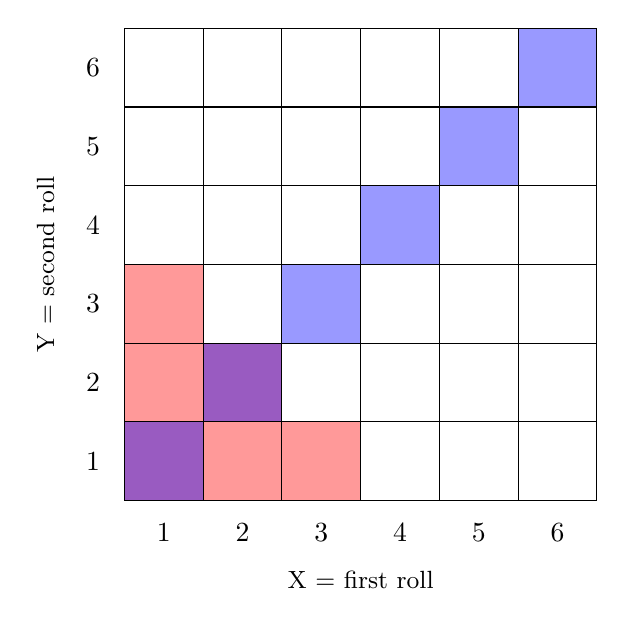
\begin{tikzpicture}
	\foreach \x in {1,...,3} {
		\fill[red!40] (0,\x-1) rectangle (4-\x,\x);
	}
	\foreach \x in {1,...,6} {
		\fill[blue,opacity=.4] (\x-1,\x-1) rectangle (\x,\x);
		\node at (\x-.5,-.4) {\x};
		\node at (-.4,\x-.5) {\x};
	}
	\draw (0,0) grid (6,6);
	\node at (3,-1) {\small X = first roll};
	\node[rotate=90] at (-1,3) {\small Y = second roll};
	\end{tikzpicture} \quad
	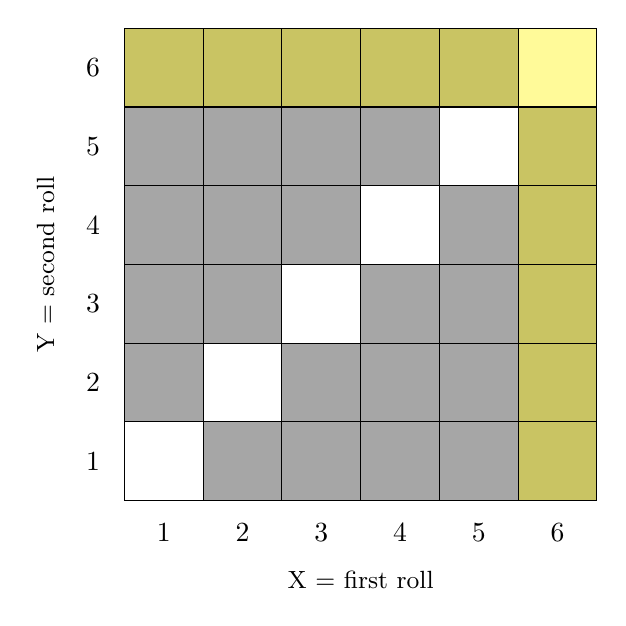
\begin{tikzpicture}
	\foreach \x in {1,...,6} {
		\fill[gray!70] (\x,\x-1) rectangle (6,\x);
		\fill[gray!70] (\x-1,\x) rectangle (\x,6);
		\node at (\x-.5,-.4) {\x};
		\node at (-.4,\x-.5) {\x};
	}
	\fill[yellow,opacity=.4] (0,5) rectangle (6,6);
	\fill[yellow,opacity=.4] (5,0) rectangle (6,5);
	\draw (0,0) grid (6,6);
	\node at (3,-1) {\small X = first roll};
	\node[rotate=90] at (-1,3) {\small Y = second roll};
	\end{tikzpicture}
\end{document} }
		\caption{On the left, the blue region shows the doubles and the red region indicates the outcomes whose sum is 4 or less; on the right, the yellow region indicates outcomes with at least one 6 and the gray region shows the outcomes where two rolls differ.}
		\label{fig:CondProbEx}
	\end{wrapfigure}
	
	Last summer, I taught myself \LaTeX\ and became a frequent user. I almost abandoned Microsoft Word completely since then and used \LaTeX\ whenever I found suitable. In fact, this file was typeset in \XeLaTeX. I am able to typeset formulae like
	\begin{align*}
	\dd x \int_{t=\sin x}^{\tan x} e^{-t^2} \dt
		&= \dd x \paren{\int_{t=0}^{\tan x} e^{-t^2} \dt -
			\int_{t=0}^{\sin x} e^{-t^2} \dt} \\
		&= \dd x \int_{t=0}^{\tan x} e^{-t^2} \dt
			- \dd x \int_{t=0}^{\sin x} e^{-t^2} \dt \\
		&= e^{-\tan^2 x} \cdot \sec^2 x - e^{-\sin^2 x} \cdot \cos x.
	\end{align*}
	With the \TikZ\ package, I could make graphics like the figure on the right.
	
	% Auditing at Fudan University
	\dots
	
	\begin{alltt}
	Work:
	\st{Study abroad service agency}
	Programming work in Starworking
	
	Study:
	MOOCing (21 MOOC courses)
	Self-learning by reading Textbooks
	Try to learn Violin, failed.
	\st{Learn LaTeX, This document was typeset in XeLaTeX. PGF/TikZ}
	Auditing at Fudan University
	\end{alltt}
	
	\section*{Intended Major and Career Plan:}
	I intend to double major in mathematics and physics. I still love computer science and there is a lot more to learn in the field. But with the double major, I do not know if I have enough time and effort for it. In addition, there are general requirements to meet.
	
	If possible, I want to skip some lower division courses in mathematics and computer science like MAT 122, MAT 221, CSC 140, CSC 151. Due to my strong interest in mathematics, I will definitely have a wonderful time with mathematics. Since I do not have much background in physics, I will probably have a very hard time with it. But I like challenges; hard courses just turn me on and easy courses are time-wasters.
	
	I want to stay in the academia and become an academic (if not a mathematician). This means I will seek master and doctoral degrees after graduation from Cornell.
	
	\section*{Term I wish to return:}
	I wish to return on Block 1 of the \onum{2016-2017} academic year.
	
	\section*{Housing Preference:}
	I do not have any particular housing preference, except that I want to make the habit of going to bed early.
	
	\nocite{*}
	
	\printbibliography
\end{document}